\documentclass[a4paper,12pt]{article}
\usepackage{graphicx}
\usepackage{verbatim}
\usepackage{amsmath}
\begin{document}
	\title{\textbf{Homework1 Rostagno}}
	\author{295706}
	\date{\today}
	\maketitle
	
	\centering \textbf{Esercizio 1}\\
	\begin{itemize}
		\item \textbf{Punto a: } 
		\begin{align*}
			U &= \{o\} & U^c &= \{a, b, c, d\} & C_U &= 6 \\
			U &= \{o, a\} & U^c &= \{b, c, d\} & C_U &= 6 \\
			U &= \{o, b\} & U^c &= \{a, c, d\} & C_U &= 8 \\
			U &= \{o, c\} & U^c &= \{a, b, d\} & C_U &= 7 \\
			U &= \{o, a, b\} & U^c &= \{c, d\} & C_U &= 7 \\
			U &= \{o, b, c\} & U^c &= \{a, d\} & C_U &= 6 \\
			U &= \{o, a, c\} & U^c &= \{b, d\} & C_U &= 7 \\
			U &= \{o, a, b, c\} & U^c &= \{d\} & C_U &= 5 \\
			\end{align*}
			Ho calcolato la capacità di ogni taglio ($C_U$) dividendo insieme di partenza (U) e insieme di arrivo ($U^c$). \\
			La capacità minima da rimuovere affinché non sia più possibile alcun flusso fattibile dal nodo $o$ al nodo $d$ è 5, va rimossa dagli archi $e_2$ $e_4$ $e_6$.
			\item \textbf{Punto b: } Sia $x$ la capacità extra da aggiungere, per poter massimizzare il throughput da o a d è necessario aggiungere la capacità su degli archi prestabiliti in un certo ordine. Dobbiamo inserire la prima unità sull'arco $e_2$, successivamente va aggiunta su $e_4$, poi su $e_1$ ed infine su $e_3$; dopodichè si ricomincia da $e_2$ e si ripete in base al valore di $x$. Questa è la sequenza che aumenta in maniera più rapida il throughput.\\
			Graficamente diventa:
			\begin{figure}[h] % L'ambiente figure permette di gestire il posizionamento
				\centering % Centra l'immagine
				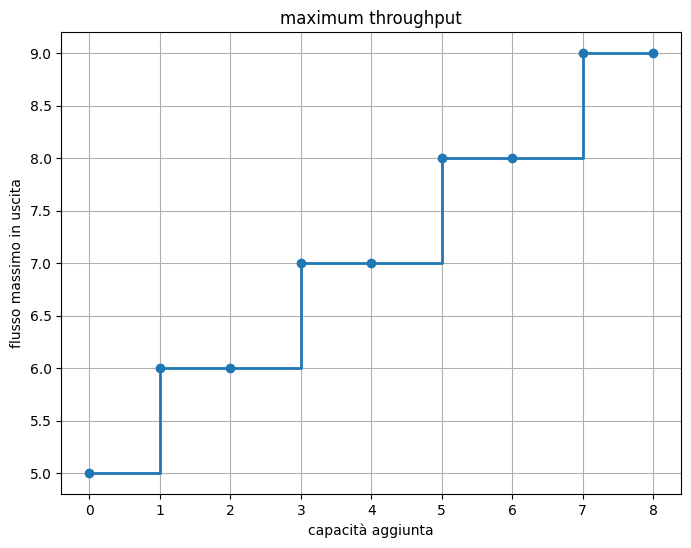
\includegraphics[width=0.8\textwidth]{graf1.png} % Inserisce l'immagine con larghezza metà pagina
				\caption{Massimo flusso in uscita in base alla capacità aggiunta} % Aggiunge una didascalia all'immagine
				\label{fig:immagine} % Aggiunge un'etichetta per riferimenti interni
			\end{figure}
			\newpage
			Nel caso in cui non si aggiunga capacità extra abbiamo come flusso max 5, se aggiungiamo una o due unità di capacità otteniamo 6 come flusso max mentre se aggiungiamo tre o quattro unità di capacità otteniamo 7 come flusso max. Dopo questi 4 valori notiamo che il grafico si ripete (come detto in precedenza).
			\item \textbf{Punto c: }Il nuovo collegamento $e_8$ di capacità 1 dovrebbe essere aggiunto in una posizione che contribuisca a migliorare il taglio minimo, di conseguenza l'ho aggiunto tra il nodo $c$ e il nodo $d$ in quanto era il collegamento più debole. La posizione delle capacità segue un andamento periodico come prima, vanno inserite in questo ordine e poi ripetute: $e_3, e_2, e_4, e_1$.
			Graficamente diventa:
			\begin{figure}[h] % L'ambiente figure permette di gestire il posizionamento
				\centering % Centra l'immagine
				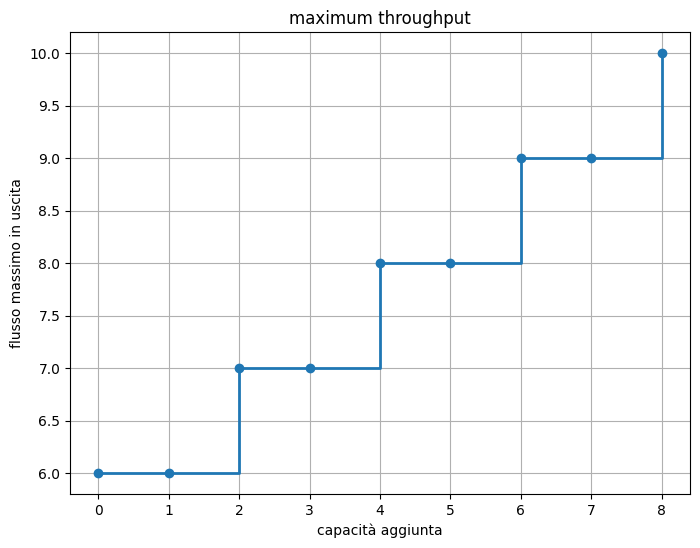
\includegraphics[width=0.8\textwidth]{graf2.png} % Inserisce l'immagine con larghezza metà pagina
				\caption{Massimo flusso in uscita in base alla capacità aggiunta} % Aggiunge una didascalia all'immagine
				\label{fig:immagine} % Aggiunge un'etichetta per riferimenti interni
			\end{figure}
			\newpage
			Notiamo che la capacità iniziale è aumentata di 1 e che dopo ogni 4 unità aggiunte il grafico si ripete.
	\end{itemize}
		\centering \textbf{Esercizio 2}\\
		\begin{itemize}
			\item \textbf{Punto a: }Considerando che il throughput è uguale a 2 e si inserisce nel vertice $o$, abbiamo tre possibili percorsi che il flusso può seguire:
			\begin{itemize}
				\item Percorso 1: $e_1, e_2, e_4$
				\item Percorso 2: $e_1, e_3, e_4$
				\item Percorso 3: $e_5, e_6$
			\end{itemize}
			Chiamiamo le nostre tre variabili di flusso $f_1f_2f_3$ dove $f_1$ rappresenta il flusso che passa per il percorso 1, $f_2$ rappresenta il flusso che passa per il percorso 2 e $f_3$ rappresenta il flusso che passa per il percorso 3. Ora scriviamo il nostro problema di ottimizzazione:\\
			\[
			\begin{aligned}
				&\min_{f_1, f_2, f_3} \quad f(x) = f_1 \cdot (5f_1+2) + f_2 \cdot (4f_2+4) + f_3 \cdot(5f_3+2) \\
				&\text{vincoli:} \\
				&f_1 + f_2 + f_3= 2, \\
				&f_1,f_2,f_3 \geq 0.
			\end{aligned}
			\]
			Facendo le opportune sostituzioni e gli opportuni calcoli si ottiene che la funzione viene minimizzata con $f=[1,0,1]$. Notiamo quindi che l'arco $e_3$ non viene utilizzato e che il flusso iniziale si divide a metà (un'unità nel percorso 1 ed un'unità nel percorso 3).\\
			Costo totale=14.
			\item \textbf{Punto b: }Per calcolare l'equilibrio di Wardrop tutti i percorsi utilizzati da almeno un utente devono avere lo stesso ritardo. Impostiamo $f_1, f_2, f_3$ i flussi di persone ch percorrono corrispettivamente il percorso 1, il percorso 2 e il percorso 3 (gli stessi definiti nel punto precedente).\\
			Ora dobbiamo eguagliare i tre ritardi e dare un vincolo ai flussi ottenendo questo sistema:\\
			\begin{equation}
				\begin{cases}
					5f_1+2=4f_2+4=5f_3+2 \\
					f_1+f_2+f_3=2
				\end{cases}
			\end{equation}
			Svolgendo i calcoli otteniamo $f_1=\frac{10}{13}$ $f_2=\frac{6}{13}$ $f_3=\frac{10}{13}$\\
			I quali rispettano tutti i vincoli del grafo.\\
			Il costo totale è $\frac{2456}{169}$. L'ho ottenuto sostituendo i valori dei vari flussi nella formula del costo totale.\\
			Il prezzo di anarchia vale $\frac{1228}{1183}=1.038$
			\item \textbf{Punto c: }Aggiungiamo un nuovo link ($e_7$) che collega il nodo $n_1$ con il nodo $n_3$.
			Otteniamo un nuovo percorso:
			\begin{itemize}
				\item Percorso 4: $e_1 e_7 e_6$
			\end{itemize}
			Indichiamo con $f_4$ il flusso che passa nel percorso 4 e risolviamo il seguente sistema.
			\begin{equation}
				\begin{cases}
					5f_1+2=4f_2+4=5f_3+2=7f_4 \\
					f_1+f_2+f_3+f_4=2
				\end{cases}
			\end{equation}
			Risolvendo il sistema a mano si ottengono questi valori di flusso:\\
			$f_1=\frac{62}{111}$,$f_2=\frac{22}{111}$,$f_3=\frac{62}{111}$,$f_4=\frac{76}{111}$\\
			Il costo totale è: $\frac{195592}{12321}=15.87$, che è maggiore del costo totale precedente(14.53), quindi abbiamo fatto verificare il paradosso di Braess. \\
			Calcoliamo ora il flusso ottimale che minimizza questa nuova rete di nodi:\\
			\newpage
				$\min_{f_1, f_2, f_3, f_4} \quad f(x) = (f_1+f_2+f_4)(3(f_1+f_2+f_4))+f_3(2f_3+2)+f_4^2+3f_2+
				f_1(f_1+1)+(f_1+f_2)(1+(f_1+f_2))+(f_3+f_4)3(f_3+f_4)$ \\
				$\textbf{vincoli:} $\\
				$f_1 + f_2+f_3+f_4 = 2$ \\
				$f_1,f_2,f_3,f_4 \geq 0$\\
				
			Dopo aver risolto in python il seguente problema di ottimizzazione otteniamo che l'ottimo è uguale al sistema precedente ovvero $f=[1,0,1,0]$ e quindi il costo totale all'ottimo è 14.\\
			Il prezzo di anarchia è dunque $\frac{195592}{12321 \cdot14}=1.134$
			\item \textbf{Punto d: }Per trovare un vettore di pedaggi ottimale $\omega$ affinchè il prezzo di anarchia sia uguale a 1, ci basta applicare la seguente formula:\\
			$\omega_e^{*}=f_e^*\tau_e'(f_e^*)$\\
			Dove $f_e^*$ sarebbero i flussi all'ottimo di sistema senza considerare i pedaggi e $\tau_e'(f_e^*)$ sarebbero le derivate delle funzioni ritardo rispetto all'ottimo di sistema.\\
			Otteniamo quindi che il vettore di pedaggi vale $\omega_e^{*}=(3,1,0,1,2,3,0)$.
			\item \textbf{Punto e: }Iniziamo a calcolare l'ottimo di sistema, ovvero il valore dei tre flussi per cui il costo totale del grafo ha valore minimo. Risolviamo il seguente problema di ottimizzazione:\\
			\[
			\begin{aligned}
				&\min_{f_1, f_2, f_3} \quad f(x) = f_1 \cdot (5f_1+2) + f_2 \cdot (2+(4+\alpha)f_2) + f_3 \cdot(5f_3+2) \\
				&\text{vincoli:} \\
				&f_1 + f_2 + f_3= \chi, \\
				&f_1,f_2,f_3 \geq 0.
			\end{aligned}
			\]
			Risolvendolo tramite il metodo del lagrangiano vincolato otteniamo i seguenti risultati:\\
			$f_1=\frac{(4+\alpha)\chi}{13+2\alpha}$ $f_2=\frac{5\chi}{13+2\alpha}$ $f_3=\frac{(4+\alpha)\chi}{13+2\alpha}$\\
			Successivamente come suggerimento indicato nel testo calcoliamo l'equilibrio di Wardrop:\\
			\begin{equation}
				\begin{cases}
					5f_1+2=(4+\alpha)f_2+2=5f_3+2 \\
					f_1+f_2+f_3=\chi
				\end{cases}
			\end{equation}
			Risolvendo il sistema otteniamo i seguenti risultati:\\
			$f_1=\frac{(4+\alpha)\chi}{13+2\alpha}$ $f_2=\frac{5\chi}{13+2\alpha}$ $f_3=\frac{(4+\alpha)\chi}{13+2\alpha}$\\
			Possiamo notare che indipendentemente da $\alpha$ e $\chi$ il prezzo di anarchia vale già 1, poichè i flussi all'equilibrio di Wardrop coincidono con i flussi all'ottimo. Di conseguenza il vettore ottimale dei pedaggi sarà $\omega_e^{*}=(0,0,0,0,0,0)$.
			\end{itemize}
\end{document}